\chapter{水库模式}\label{水库模式}
%\addcontentsline{toc}{chapter}{陆地表面的水分循环}
\begin{mymdframed}{代码}
  本章对应的代码文件为\texttt{CaMa/src/cmf\_ctrl\_damout\_mod.F90}。
\end{mymdframed}
本模块在CaMa-Flood中实施水库运行方案,通过识别坝体所在的集水区单元,根据水库运行规则计算水库流出量,构建考虑大坝影响的河道汇流参数化方案,以刻画水库对陆面水文循环过程的影响。

\section{水库调度规则参数化方案}
在大尺度陆面模式中进行水库扰动模拟,需要对水库的调度规则进行一定的假设和概化,现有方案大致可分为三类:基于入流和需求的调度方案、基于目标库容的分段调度方案和基于离线优化的调度方案\citep{yassin2019representation},其中以前两种方法应用最为广泛。本版本已加入目前陆面模式中采用的主流水库调度参数化方案,如表~\ref{tab:水库模块可选水库调度方案} 所示,可通过相应的方案代码进行调用。

\begin{table}[htbp]
  \centering
  \caption{水库模块可选水库调度方案}
  \label{tab:水库模块可选水库调度方案}
  \begin{tabular}{cc>{\centering\arraybackslash}p{5.5cm}}
    \toprule
    方案类型                                     & 方案代码 & 代表模式                                    \\ \midrule
    \multirow[b]{2}{*}{基于入流和需求的调度方案} & H06      & H08, WaterGAP, WBMplus, MATSIRO, DBH, LPJmL \\ \cline{2-3}
                                                 & V13      & MOSART‐WM                                   \\
    \hline
    \multirow{2}{*}{基于目标库容的分段调度方案}  & LIS      & LISFLOOD, CWatM                             \\ \cline{2-3}
                                                 & H22      & CAMA-Flood                                  \\
    \bottomrule
  \end{tabular}
\end{table}

\subsection{H06方案}
H06表示~\citet{hanasaki2006reservoir}提出的基于入流和需求的调度方案,该方案根据水库用途、水库初始库容、水库最大库容、模拟入流量和下游需水量等信息,分别为灌溉水库和非灌溉水库(除灌溉之外的用途均为非灌溉)设定调度规则,计算公式如下:
\begin{equation}
  Q_{\mathrm{out}}=\begin{cases}
    k_{\mathrm{rls}} \times Q_{\mathrm{out}}^{'}, & \quad c \geqslant 0.5 \\
    R \times k_{\mathrm{rls}} \times Q_{\mathrm{out}}^{'}+\left(1-R\right) \times Q_{\mathrm{in}}, & \quad c<0.5
  \end{cases}
\end{equation}
%
其中:
\begin{equation}
  \begin{cases}
    \text{灌溉水库,} Q_{\mathrm{out}}^{'}= \begin{cases}
      Q_{\mathrm{n}}+D-\overline{D}, &\quad DPI<(1-M)\\
      Q_{\mathrm{n}} \times \left(M+\frac{\left(1-M\right)D}{\overline{D}}\right), &\quad DPI \geqslant (1-M)
    \end{cases}\\
    \text{非灌溉水库,} Q_{\mathrm{out}}^{'}=Q_{\mathrm{n}}
  \end{cases}
\end{equation}

上式中变量和参数的含义如表~\ref{tab:H06方案变量参数表} 所示。

\begin{table}[htbp]
  \centering
  \caption{H06方案中的变量和参数的含义}
  \label{tab:H06方案变量参数表}
  \begin{threeparttable}
    \begin{tabular}{ccc}
      \toprule
      名称               & 含义/计算方法                                                            & 量纲                \\ \midrule
      $Q_{\mathrm{out}}$ & 水库出流量[变量]                                                         & [\unit{L^3.T^{-1}}] \\
      $Q_{\mathrm{in}}$  & 水库入流量[变量]                                                         & [\unit{L^3.T^{-1}}] \\
      $D$                & 当日需水量[变量]                                                         & [\unit{L^3.T^{-1}}] \\
      $Q_{\mathrm {n}} $ & 水库多年平均正常流量[参数]                                               & [\unit{L^3.T^{-1}}] \\
      $\overline{D}$     & 多年平均日需水量[参数]                                                   & [\unit{L^3.T^{-1}}] \\
      $M$                & 最小需求满足系数[参数]                                                   & [-]                 \\
      $DPI$              & 年平均需求量与年平均水库入流量的比值[参数]                               & [-]                 \\
      $k_{\mathrm{rls}}$ & 释放系数[参数],$k_{\mathrm{rls}} = \frac{V_0}{\alpha V_{\mathrm {t}} }$ & [-]                 \\
      $R$                & 需求决定系数[参数],$R=\min(1, \alpha c)$                                & [-]                 \\
      $\alpha$           & 无量纲常数[参数]                                                         & [-]                 \\
      $c$                & 总库容量与年总水库入流量的比值[参数]                                     & [-]                 \\
      $V_0$              & 初始蓄水量[参数]                                                         & [\unit{L^3}]        \\
      $V_{\mathrm {t}} $ & 水库最大库容[参数]                                                       & [\unit{L^3}]        \\
      \bottomrule
    \end{tabular}
    \begin{tablenotes}
      \footnotesize
    \item[注:] 原 H06 方案中 $R=\min(1,4 c^2)$,\citet{Shin-etal_19} 将该参数的计算修改为 $R=\min(1,\alpha c)$,以修正原方案导致库容模拟不稳定的问题。
    \end{tablenotes}
  \end{threeparttable}
\end{table}

\subsection{V13方案}
V13表示~\citet{voisin2013improved}提出的调度方案,在H06方案的基础上增加了防洪期以同时实现防洪和灌溉目标。该方案根据水库多年平均入库流量的季节变化,定义了三个特征时刻:NDFC表示防洪期结束月,为运营期开始前的湿润期的第一个月;STFC表示防洪期开始月,为运营期开始前的枯水期内流量最低的月份;STOp表示运营期的开始月,\citet{hanasaki2006reservoir}将运营期的开始定义为长期平均月流量低于长期平均年流量的第一个月。
在STFC到NDFC时段内,V13方案在H06方案的基础上增加额外的出流,从而使水库为汛期的到来留出更多库容,在原V13方案中该时段内每个时刻的额外出流:
\begin{equation}
  drop = \frac{\sum_{i = \text{STFC}}^{\text{NDFC} - 1}{{(Q}_{\text{in}}^{i} - Q_{\mathrm{n}})}}{\left( \text{NDFC} - \text{STFC} \right)}
\end{equation}
该方案为回溯性方案,如不选择回溯性方案,可将额外出流简化为:
\begin{equation}
  drop = \left| Q_{\text{in}}^{i} - Q_{\mathrm{n}} \right|
\end{equation}
在NDFC到STOp时段内,通过只释放年平均流量$Q_{\mathrm{n}}$来确保水库为灌溉季节再次蓄水。

\subsection{LIS方案}
LIS表示LISFLOOD所采用的基于目标库容的分段调度方案(\url{https://ec-jrc.github.io/lisflood-model/3\_03\_optLISFLOOD\_reservoirs/}),计算公式如下:
\begin{equation}
  \begin{aligned}
    F > L_{\mathrm{f}}, \quad &Q_{\mathrm{out}}=\max\left[Q_{\mathrm{max}},\ (F-L_{\mathrm{f}}-0.01) \times \frac{V_{\mathrm {t}} }{\Delta t}\right] \\
    \quad &Q_{\mathrm{max}} = \min\left[Q_{\mathrm{f}},\ {\max(1.2 \times Q_{\mathrm{in}},Q_{\mathrm{adj,n}})}\right]
  \end{aligned}
\end{equation}
\begin{equation}
  L_{\mathrm{adj,f}} < F < L_{\mathrm{f}}, \quad Q_{\mathrm{out}}=Q_{\mathrm{adj,n}}+\left(Q_{\mathrm{f}}-Q_{\mathrm{adj,n}}\right) \times \frac{F-L_{\mathrm{adj,f}}}{L_{\mathrm{f}}-L_{\mathrm{adj,f}}}
\end{equation}
\begin{equation}
  L_{\mathrm{n}} < F < L_{\mathrm{adj,f}}, \quad Q_{\mathrm{out}}=Q_{\mathrm{adj,n}}
\end{equation}
\begin{equation}
  2L_{\mathrm{c}} < F < L_{\mathrm{n}}, \quad Q_{\mathrm{out}}=Q_{\mathrm{min}}+\left(Q_{\mathrm{adj,n}}-Q_{\mathrm{min}}\right) \times \frac{F-2L_{\mathrm{c}}}{L_{\mathrm{n}}-2L_{\mathrm{c}}}
\end{equation}
\begin{equation}
  F < 2L_{\mathrm{c}}, \quad Q_{\mathrm{out}}=\min\left[Q_{\mathrm{min}}, \frac{V_{\mathrm {t}} }{\Delta t}\right]
\end{equation}
如果出现$F<L_{\mathrm{f}}$且$Q_{\mathrm{out}}>\min(1.2 \times Q_{\mathrm{in}},\ Q_{\mathrm{adj,n}})$,则对水库出流结果进行以下修正:
\begin{equation}
  Q_{\mathrm{out}} = \min\left[Q_{\mathrm{out}}, \max(Q_{\mathrm{in}}, Q_{\mathrm{adj,n}})\right]
\end{equation}
上式中变量和参数的含义如表~\ref{tab:LIS方案变量参数表} 所示。

\begin{table}[htbp]
  \centering
  \caption{LIS方案中的变量和参数的含义}
  \label{tab:LIS方案变量参数表}
%    \begin{threeparttable}
  \begin{tabular}{ccc}
    \toprule
    名称                 & 含义/计算方法                                                               & 量纲                \\ \midrule
    $Q_{\mathrm{out}}$   & 水库出流量[变量]                                                            & [\unit{L^3.T^{-1}}] \\
    $Q_{\mathrm{in}}$    & 水库入流量[变量]                                                            & [\unit{L^3.T^{-1}}] \\
    $V$                  & 水库实时蓄水量[变量]                                                        & [\unit{L^3}]        \\
    $F$                  & 实时蓄水系数[变量], $F=\frac{V}{V_{\mathrm{t}}}$                            & [-]                 \\
    $L_{\mathrm{f}}$     & 防洪库容系数[参数], $L_{\mathrm{f}}=\frac{V_{\mathrm{f}}}{V_{\mathrm{t}}}$  & [-]                 \\
    $L_{\mathrm{n}}$     & 正常库容系数[参数], $L_{\mathrm{n}}=\frac{V_{\mathrm{n}}}{V_{\mathrm{t}}}$  & [-]                 \\
    $L_{\mathrm{c}}$     & 保留库容系数[参数], $L_{\mathrm{c}}=\frac{V_{\mathrm{c}}}{V_{\mathrm{t}}}$  & [-]                 \\
    $L_{\mathrm{adj,f}}$ & \makecell{调整防洪库容系数[参数],                                         \\
    $L_{\mathrm{adj,f}} = L_{\mathrm{n}}+AdjL_{\mathrm{n}} \times \left(L_{\mathrm{f}}-L_{\mathrm{n}}\right)$}
                         & [-]                                                                        \\
    $AdjL_{\mathrm{n}}$  & 无量纲调整系数[参数],取值$\left(0,1\right)$                                & [-]                 \\
    $Q_{\mathrm{f}}$     & 防洪流量[参数]                                                              & [\unit{L^3.T^{-1}}] \\
    $Q_{\mathrm{n}}$     & 正常流量[参数]                                                              & [\unit{L^3.T^{-1}}] \\
    $Q_{\mathrm{min}}$   & 最小环境流量[参数]                                                          & [\unit{L^3.T^{-1}}] \\
    $Q_{\mathrm{adj,n}}$ & \makecell{调整正常流量[参数],                                             \\
    $Q_{\mathrm{adj,n}}=\max(Q_{\mathrm{min}},\,\min(AdjQ_{\mathrm{n}} \times Q_{\mathrm{n}},\,Q_{\mathrm{f}}))$}
                         & [\unit{L^3}]                                                               \\
    $AdjQ_{\mathrm{n}}$  & 无量纲调整系数[参数],取值$\left(0.25,2\right)$                             & [-]                 \\
    \bottomrule
  \end{tabular}
%    \end{threeparttable}
\end{table}

\subsection{H22方案}
H22表示~\citet{hanazaki2022development}提出的调度方案,根据水库入流量和实时库容大小,调节出库流量以削减汛期峰值流量,控制出库流量不超过防洪流量,且根据汛期发展时段调整出流系数,计算公式如下:
\begin{equation}
  V_{\mathrm{e}} < V < V_{\mathrm{t}}, \quad Q_{\mathrm{out}} = \max(Q_{\mathrm{f}},\, Q_{\text{in}})\
\end{equation}
\begin{equation}
  V_{\mathrm{f}}<V<V_{\mathrm{e}},\ Q_{\mathrm{out}} = \begin{cases}
    Q_{\mathrm{f}}+k \times \frac{V-V_{\mathrm{c}}}{V_{\mathrm{e}}-V_{\mathrm{c}}} \times \left[(Q_{\mathrm{in}}-Q_{\mathrm{f}})\right], & \quad Q_{\mathrm{in}} > Q_{\mathrm{f}}\\
    0.5Q_{\mathrm{n}}+k \times \left(\frac{V-V_{\mathrm{c}}}{V_{\mathrm{e}}-V_{\mathrm{c}}}\right)^2 \times (Q_{\mathrm{f}}-Q_{\mathrm{n}}), & \quad Q_{\mathrm{in}} < Q_{\mathrm{f}}
  \end{cases}
\end{equation}
\begin{equation}
  V_{\mathrm{c}}<V<V_{\mathrm{f}},\ Q_{\mathrm{out}} = \begin{cases}
    0.5Q_{\mathrm{n}}+k \times \frac{V-V_{\mathrm{c}}}{V_{\mathrm{f}}-V_{\mathrm{c}}} \times \left[(Q_{\mathrm{f}}-Q_{\mathrm{n}})\right], & \quad Q_{\mathrm{in}} > Q_{\mathrm{f}} \\
    0.5Q_{\mathrm{n}}+k \times \left(\frac{V-V_{\mathrm{c}}}{V_{\mathrm{e}}-V_{\mathrm{c}}}\right)^2 \times (Q_{\mathrm{f}}-Q_{\mathrm{n}}), & \quad Q_{\mathrm{in}} < Q_{\mathrm{f}}
  \end{cases}
\end{equation}
\begin{equation}
  V < V_{\mathrm{c}}, \quad Q_{\mathrm{out}} = Q_{\mathrm{n}} \times \frac{V}{V_{\mathrm{f}}}
\end{equation}
上式中变量和参数的含义如表~\ref{tab:H22方案变量参数表} 所示。

\begin{table}[htbp]
  \centering
  \caption{H22方案中的变量和参数的含义}
  \label{tab:H22方案变量参数表}
%    \begin{threeparttable}
  \begin{tabular}{ccc}
    \toprule
    名称                                                                & 含义/计算方法                   & 量纲                \\ \midrule
    $Q_{\mathrm{out}}$                                                  & 水库出流量[变量]                & [\unit{L^3.T^{-1}}] \\
    $Q_{\mathrm{in}}$                                                   & 水库入流量[变量]                & [\unit{L^3.T^{-1}}] \\
    $V$                                                                 & 水库实时蓄水量[变量]            & [\unit{L^3}]        \\
    $V_{\mathrm{t}}$                                                    & 最大库容[参数]                  & [\unit{L^3}]        \\
    $V_{\mathrm{e}}$                                                    & 警戒库容[参数]                  & [\unit{L^3}]        \\
    $V_{\mathrm{f}}$                                                    & 防洪库容[参数]                  & [\unit{L^3}]        \\
    $V_{\mathrm{c}}$                                                    & 保留库容[参数]                  & [\unit{L^3}]        \\
    $Q_{\mathrm{f}}$                                                    & 防洪流量[参数]                  & [\unit{L^3.T^{-1}}] \\
    $Q_{\mathrm{n}}$                                                    & 正常流量[参数]                  & [\unit{L^3.T^{-1}}] \\
    $K$                                                                 & \makecell{出流调节系数[参数], \\
    取值$\max\left(1-\frac{V_{\mathrm{t}}-V_{\mathrm{f}}}{A},0\right)$} & [-]                            \\
    $A$                                                                 & 水库汇流面积[参数]              & [\unit{L^2}]        \\
    \bottomrule
  \end{tabular}
%    \end{threeparttable}
\end{table}

\section{考虑大坝影响的河道汇流参数化方案}
相比自然河道的汇流方案,考虑大坝影响的汇流方案存在以下改动:当河道中存在大坝时,由于水的连续流动和河道的水力连结被切断,在与大坝网格紧连的下游网格处,圣维南动力方程中的局部加速项和静水压力项被忽略,在使用局部惯性方程(CaMa-Flood中使用的默认算法)进行一般计算后,使用运动波动方程重新计算流量。在下一步中,将来自上游河网的所有流出汇总为水库流入,并根据重新计算的流入和蓄水量确定水库流出。
\begin{equation}
  {\mathrm g} A \frac{\partial z}{\partial x}+\frac{{\mathrm g} n^{2}|Q| Q}{R_{\mathrm{H}}^{4 / 3} A}=0
\end{equation}
式中变量含义同章节~\ref{诊断洪泛状态} 所述。


此外,由于大坝对汇流过程的拦截作用,在计算大坝网格下游格点的河道蓄水和淹没时,质量连续方程中的汇流网格和汇流面积将不再包括大坝网格上游的部分,且与大坝网格紧连的下游网格其入流径流量替换为水库出流量。
\begin{equation}
  S_{i}^{t+\Delta t}=S_{i}^{t}+\sum_{k}^{Upstream-2} Q_{k}^{t} \Delta t-Q_{i}^{t} \Delta t+A c_{i} R_{i}^{t} \Delta t
\end{equation}
式中$Upsteam-2$表示在原上游网格的基础上除去大坝上游网格 (例如图~\ref{fig:大坝对下游河道汇流计算方案的影响示意图} 所示),其他变量含义同章节~\ref{诊断洪泛状态} 所述。

{
  \begin{figure}[htbp]
    \centering
    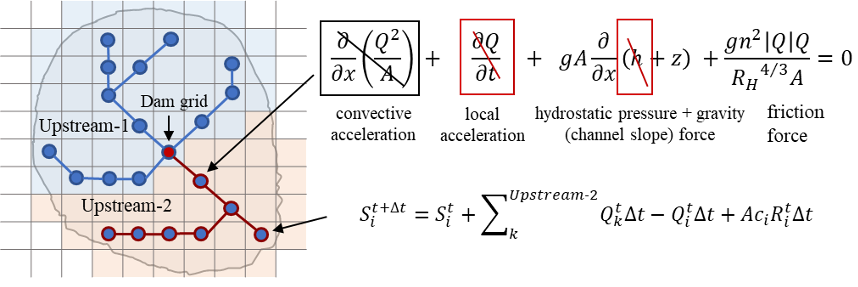
\includegraphics{Figures/陆地表面的水分循环/大坝对下游河道汇流计算方案的影响示意图.png}
    \caption{大坝对下游河道汇流计算方案的影响示意图}
    \label{fig:大坝对下游河道汇流计算方案的影响示意图}
  \end{figure}
}
